\documentclass[12pt,a4paper]{article}
\usepackage[latin1]{inputenc}
\usepackage{amsmath}
\usepackage{amsfonts}
\usepackage{amssymb}
\usepackage{graphicx}
\usepackage{tikz}
\usetikzlibrary{bayesnet}
\usepackage{bm}
\author{}
\title{}
\begin{document}
	\date{}
	\maketitle
	\centering
	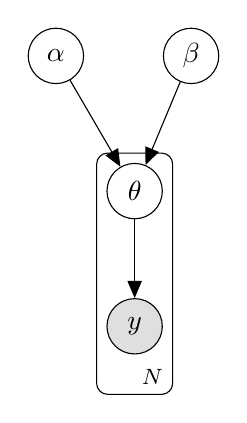
\begin{tikzpicture}
%	\node[obs] (y) {$y_t$};
%	\node[latent, right = of y]  (sig_y) {$\sigma^2_y$};
%	\node[obs, left = of y] (t) {$t_i$};
%	\node[const, above = of y] (C) {$C(t)$};
%
%	
%	\node[latent, above = of C, xshift = -2 cm]  (V) {$V$};
%	\node[obs, left = of C]  (X) {$\mathbf{x}$};
%	\node[latent, above = of V, xshift = 0.5 cm]  (sig_V) {$\sigma^2_{V}$};
%	\node[latent, above = of V, xshift = -0.5 cm]  (beta) {$\beta$};
%	
%	\node[latent, above = of C, xshift = 0 cm]  (k) {$k$};
%	\node[latent, above = of k, xshift = 0.5 cm]  (sig_k) {$\sigma^2_{k}$};
%	\node[latent, above = of k, xshift = -0.5 cm]  (beta_k) {$\beta_k$};
%	
%	\node[latent, above = of C, xshift = 2 cm]  (k_a) {$k_a$};
%	\node[latent, above = of k_a, xshift = 0.5 cm]  (sig_k_a) {$\sigma^2_{k_a}$};
%	\node[latent, above = of k_a, xshift = -0.5 cm]  (beta_k_a) {$\beta_{k_a}$};
%	
%	%edges
%	\edge{beta,X,sig_V}{V};
%	\edge{X}{k,k_a};
%	\edge{V,k,k_a}{C};
%	\edge{t}{y};
%	\edge{C,sig_y}{y};	
%	\edge{beta_k, sig_k}{k};
%	\edge{beta_k_a, sig_k_a}{k_a};
%	
%	
%	%Plates
%	 \plate {time} {(y)(t)} {$i = 1 \dots 8$} ; %
%	 \plate {patients} {(time)(X)(V)(C)(k)(k_a)} {$N = 1 \dots 36$} ; %

	\node[latent, xshift = -1.0 cm] (a) {$\alpha$};
	\node[latent, right = of a]  (b) {$\beta$};
	\node[latent, below = of a, xshift = 1.0 cm]  (theta) {$\theta$};
	\node[obs, below = of theta](y){$y$};
	
	\edge{a,b}{theta};
	\edge{theta}{y};
	
	\plate{exp}{(theta)(y)}{$N$};
	\end{tikzpicture}
	
	

\end{document}